\documentclass[]{scrartcl}

\usepackage{amsmath}
\usepackage{amssymb}
\usepackage[utf8]{inputenc}
\usepackage[T1]{fontenc}
\usepackage{lmodern}
\usepackage{ngerman}
\usepackage{geometry}
\usepackage{graphicx}
\usepackage{wrapfig}
\usepackage{caption}
\usepackage{wasysym}
\usepackage{siunitx}
\usepackage{picinpar}
\usepackage{tikz}
\usepackage{float}
\usepackage{booktabs}

\renewcommand{\figurename}{Abb.}
\usepackage[
	colorlinks=true,
	urlcolor=blue,
	linkcolor=black
]{hyperref}


%Hier Titel und so
\newcommand{\versuchnummer}{V59} 
\newcommand{\versuchname}{Modulation und Demodulation elektrischer Schwingungen} 
\newcommand{\versuchdatum}{24.02.16} 


\title{Versuch \versuchnummer\\ \versuchname}
\subtitle{Physikalisches Fortgeschrittenenpraktikum}
\author{Robert Rauter und Björn Lindhauer}
\date{\versuchdatum} 
\begin{document}
\begin{titlepage}
{\large \versuchdatum}
\vspace{7cm}
\begin{center}
\textbf{\huge Versuch \versuchnummer:}\\
\vspace{0.5cm}
\textbf{\huge \versuchname}\\
\vspace{0.2cm}
\textbf{ Physikalisches Fortgeschrittenenpraktikum}\\
\vspace{9cm}

{\Large Robert Rauter \ \ \hspace{1.5cm} und \hspace{1.5cm} Björn Lindhauer}\\
{ \url{robert.rauter@tu-dortmund.de} \ \ \hspace{2cm} \url{bjoern.lindhauer@tu-dortmund.de}}
\end{center}
\end{titlepage}
\section{Einleitung}

\section{Theoretische Grundlagen}
\subsection{Ideale Operationsverstärker}
Ein Operationsverstärker wird durch das Schaltsymbol XXXX repräsentiert und ist ein elektronisches Bauteil, dessen Ausgangsspannung
\begin{align}
 U_{\text{A}}=V\cdot \left( U_{\text{P}}-U_{\text{N}} \right)
\end{align}
ist, welche somit proportional zur Differenz an den beiden Eingängen ist.

Deswegen wir er auch als gleichstromgekoppelter Differenzverstärker bezeichnet.

Die Betribsspannung $\pm U_{\text{B}}$ limitiert das Ausgangssignal $U_{\text{A}}$ auf dem Bereich
\begin{align}
 -U_{\text{B}} < U_{\text{A}} < U_{\text{B}}
\end{align}
und sorgt für eine Sättigung bei $\left| U_{\text{A}} \right| > U_{\text{B}}$. Der Verlauf der Kurve ist in Abbildung XXX schematisch dargestellt. 

Es wird der Eingang mit der Spannung $U_{\text{P}}$ als nicht-invertierter Eingang (+) bezeichnet, da die Ausgangsspannung $U_{\text{A}}$ n Phase mit der Spannung $U_{\text{P}}$ ist.
Die Ausgangsspannung ist jedoch gegenphasig zur Spannung $U_{\text{N}}$, weshalb deren Eingang als invertierter Eingang (-) bezeichnet wird.

Bei einem idealen Operationsverstärker ist die Leerlaufverstärkung $V$, sowie der Eingangswiderstand $r_{e}$ unendlich groß und der Ausgangswirderstand $r_a$ verschwindet.

Dies ist beim realen Operationsverstärker jedoch nicht der Fall, sodass es sinnvoll ist, weitere Größen zu definieren.

\subsection{Reale Operationsverstärker}
Die Ausgangsspannung ist von Null verschieden, wenn die beiden Eingangsspannungen gleich sind. Deshalb wird die Gleichtaktverstärkung
\begin{align}
 V_{gl}:=\frac{\Delta U_{A}}{\Delta U_{gl}}
\end{align}
definiert.

Aus den endlichen Eingangswiderständen folgen Eingangsruheströme $I_{P}$ und $I_{N}$, die zur Definition des Eingangsruhestroms
\begin{align}
 I_{B}:=\frac{1}{2} \cdot \left(I_{P}+I_{N}\right)
\end{align}
und des Offsetstroms
\begin{align}
 I_{0}:= \left. I_{P}-I_{N}\right|_{U_{P}=U_{N}=0} 
\end{align}
führen.

Der Differenzwiderstand wird als
\begin{align}
 r_{D}:=\left\lbrace 
\begin{array}{ll}
\frac{\Delta U_{P}}{\Delta I_{P}} & \text{, }U_{N}=0 \vspace{0.2cm}\\
\frac{\Delta U_{N}}{\Delta I_{N}} & \text{, }U_{P}=0
\end{array}
\right\rbrace 
\end{align}
definiert und der Gleichtakteingangswiderstand als
\begin{align}
 r_{gl}:=\frac{\Delta U_{gl}}{\Delta I_{gl}} \hspace{0.3cm}\text{.}
\end{align}

Da die Ausgangsspannung $U_{a}$ bei realen Operationsverstärkern ungleich null ist, wird die Offsetspannung
\begin{align}
 U_0:=\left. U_{P}-U_{N} \right|_{U_{a}=0}
\end{align}
definiert.

Diese ist häufig eine Funktion der Temperatur, Zeit und Betriebsspannung. Die totale Ableitung von $U_{0}$ wird Offsetspannungsdrift genannt.

Reale Operationsverstärker kommen idealen Operationsverstärkern sehr nahe, sodass die eingeführten Größen als Störparameter angesehen werden können und somit zu Korrekturen führen.


\section{Durchführung}

\subsection{Frequenzgang des gegengekoppelten Verstärkers}

\subsection{Der Umkehrintegrator}

\subsection{Der Umkehrdifferentiator}

\subsection{Der Schmitt-Trigger}

\subsection{Der Dreiecksgenerator}

\subsection{Die Schwingungsdifferentialschaltung}

\subsection{Phasenbeziehung des gegengekoppelten Verstärkers}

\section{Auswertung}

\subsection{Frequenzgang des gegengekoppelten Verstärkers}

In den Abbildungen \ref{fig:freq1}-\ref{fig:freq4} sind die Frequenzgänge des gegengekoppelten Verstärkers für verschiedene Verstärkungsgrade $V'$ dargestellt. Es wurde dabei stets ein Widerstand der Größe $R_1=\SI{1}{\kilo\ohm}$ verwendet. \\
\begin{minipage}[t]{0.5\textwidth}
	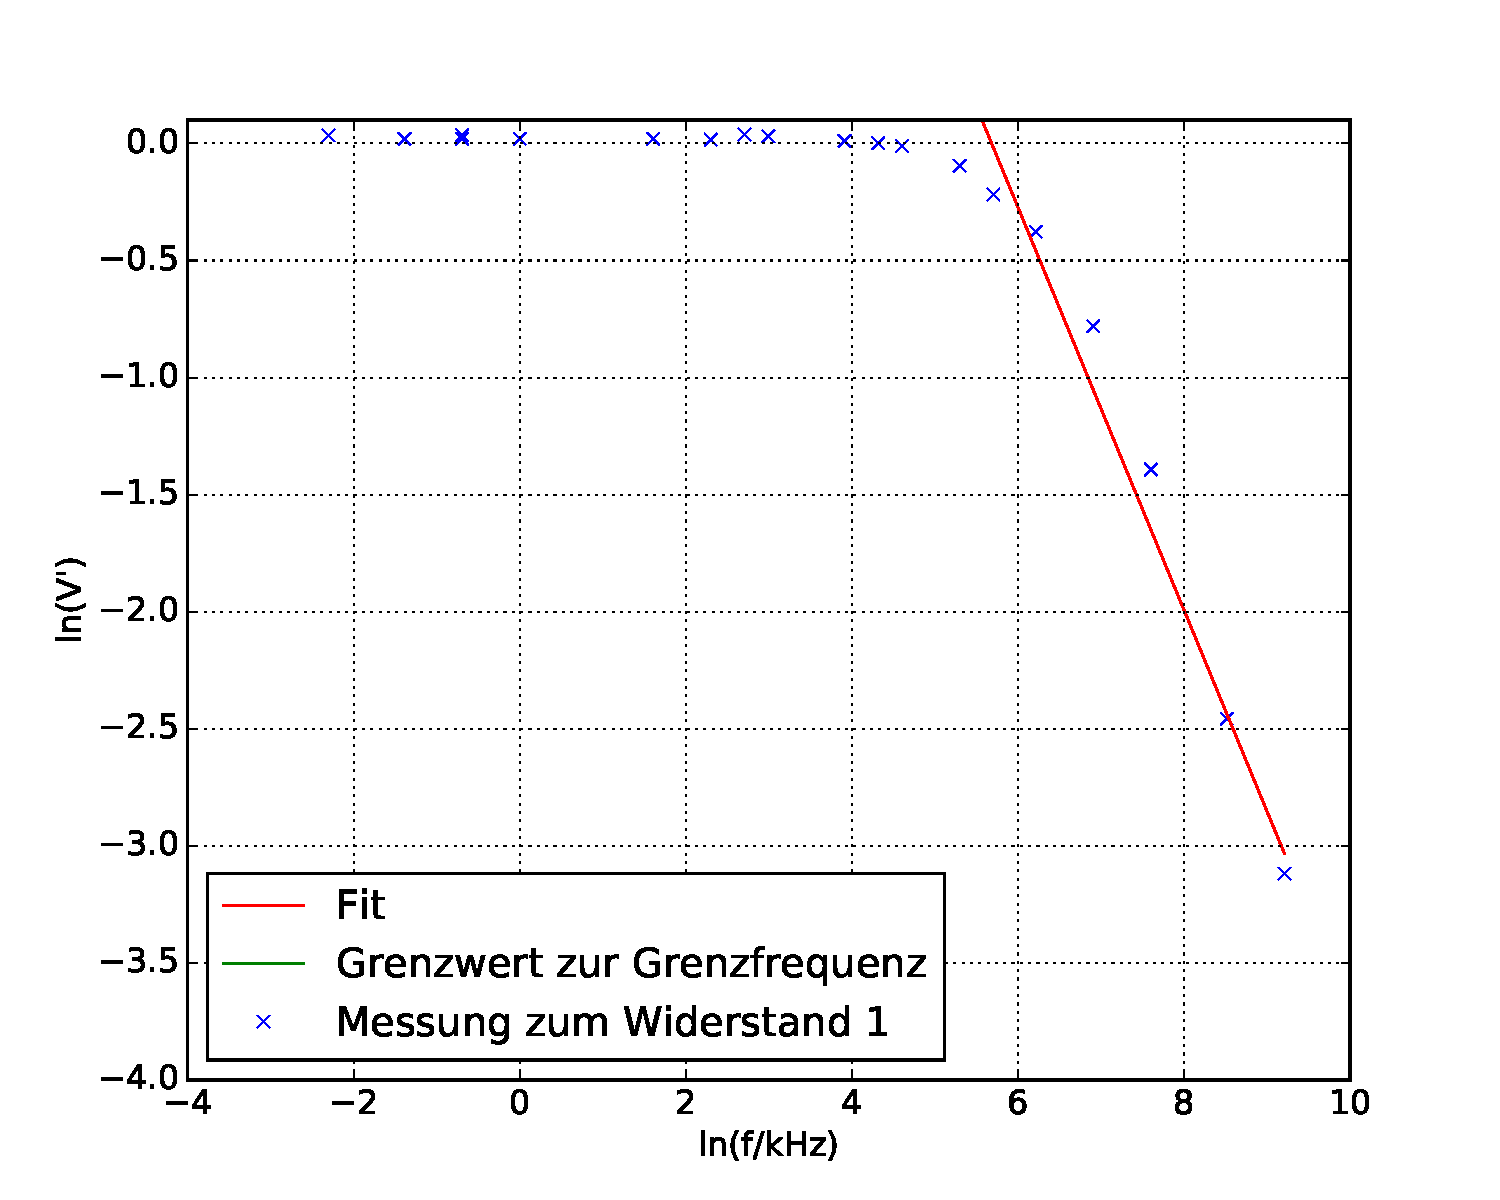
\includegraphics[width=\textwidth]{images/plot1.pdf}
	\captionof{figure}{Frequenzgang für R$_n=\SI{1}{\kilo\ohm}$}
	\label{fig:freq1}
\end{minipage}
\begin{minipage}[t]{0.5\textwidth}
	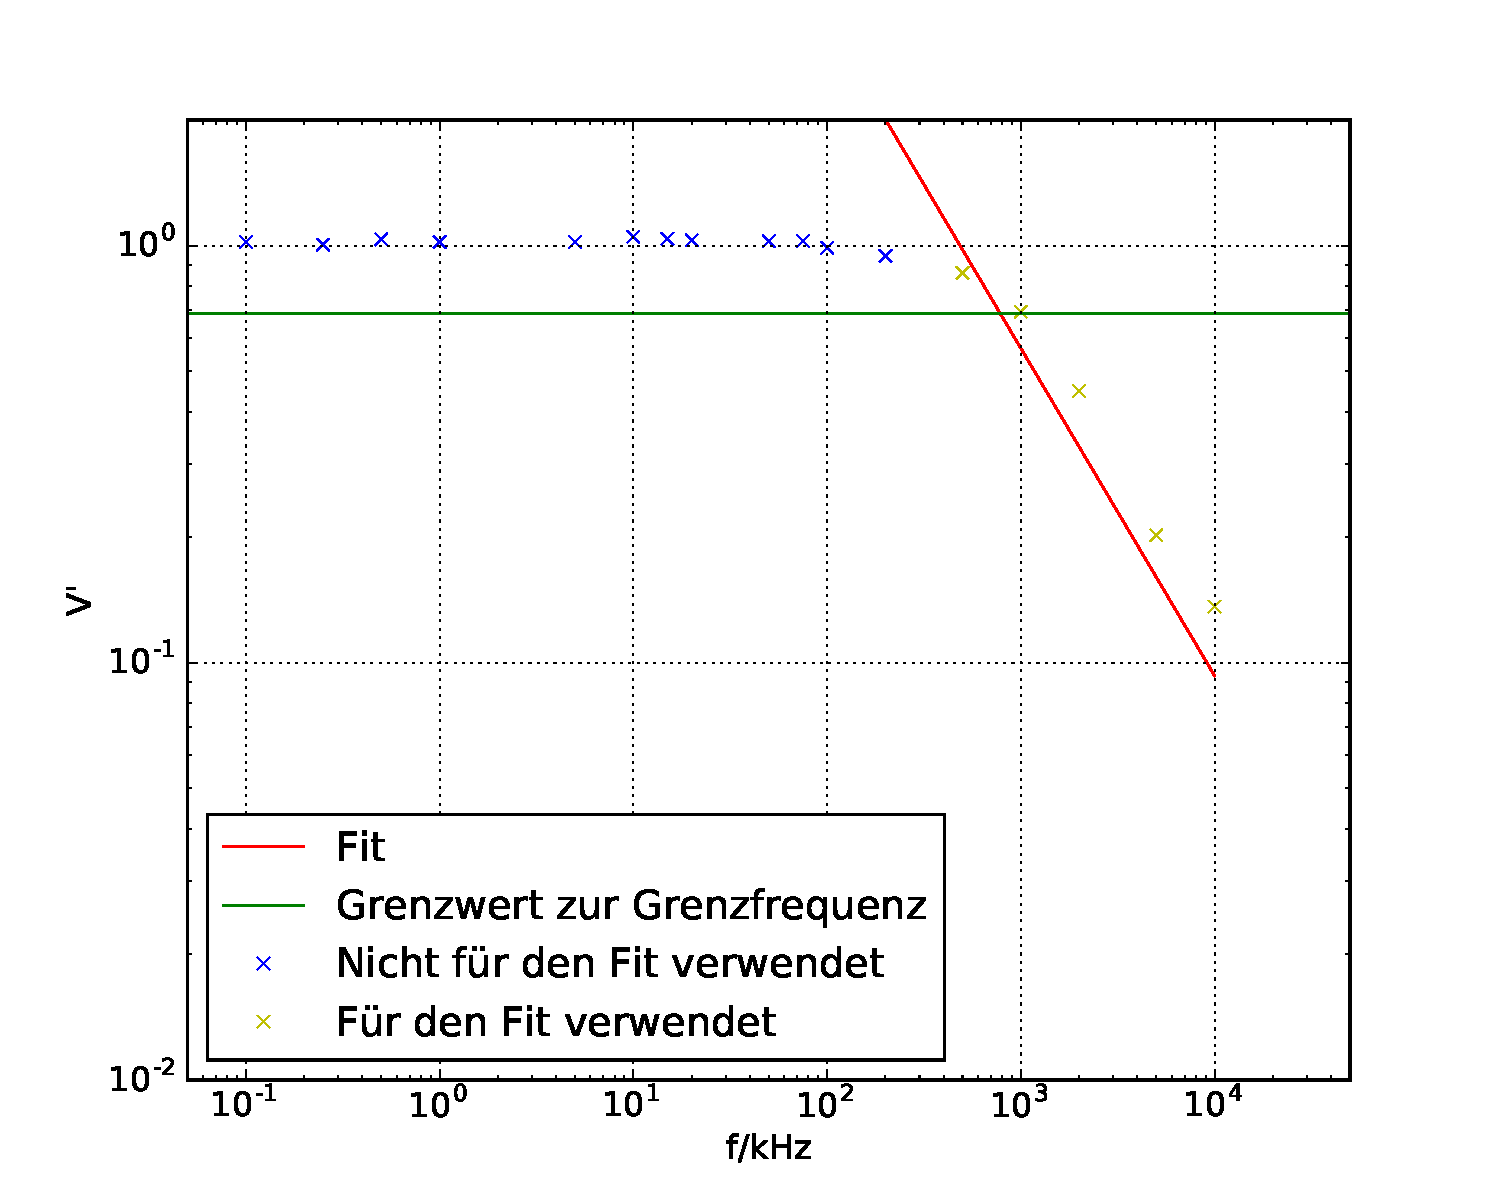
\includegraphics[width=\textwidth]{images/plot2.pdf}
	\captionof{figure}{Frequenzgang für R$_n=\SI{100}{\ohm}$}
\end{minipage} \\
\begin{minipage}[t]{0.5\textwidth}
	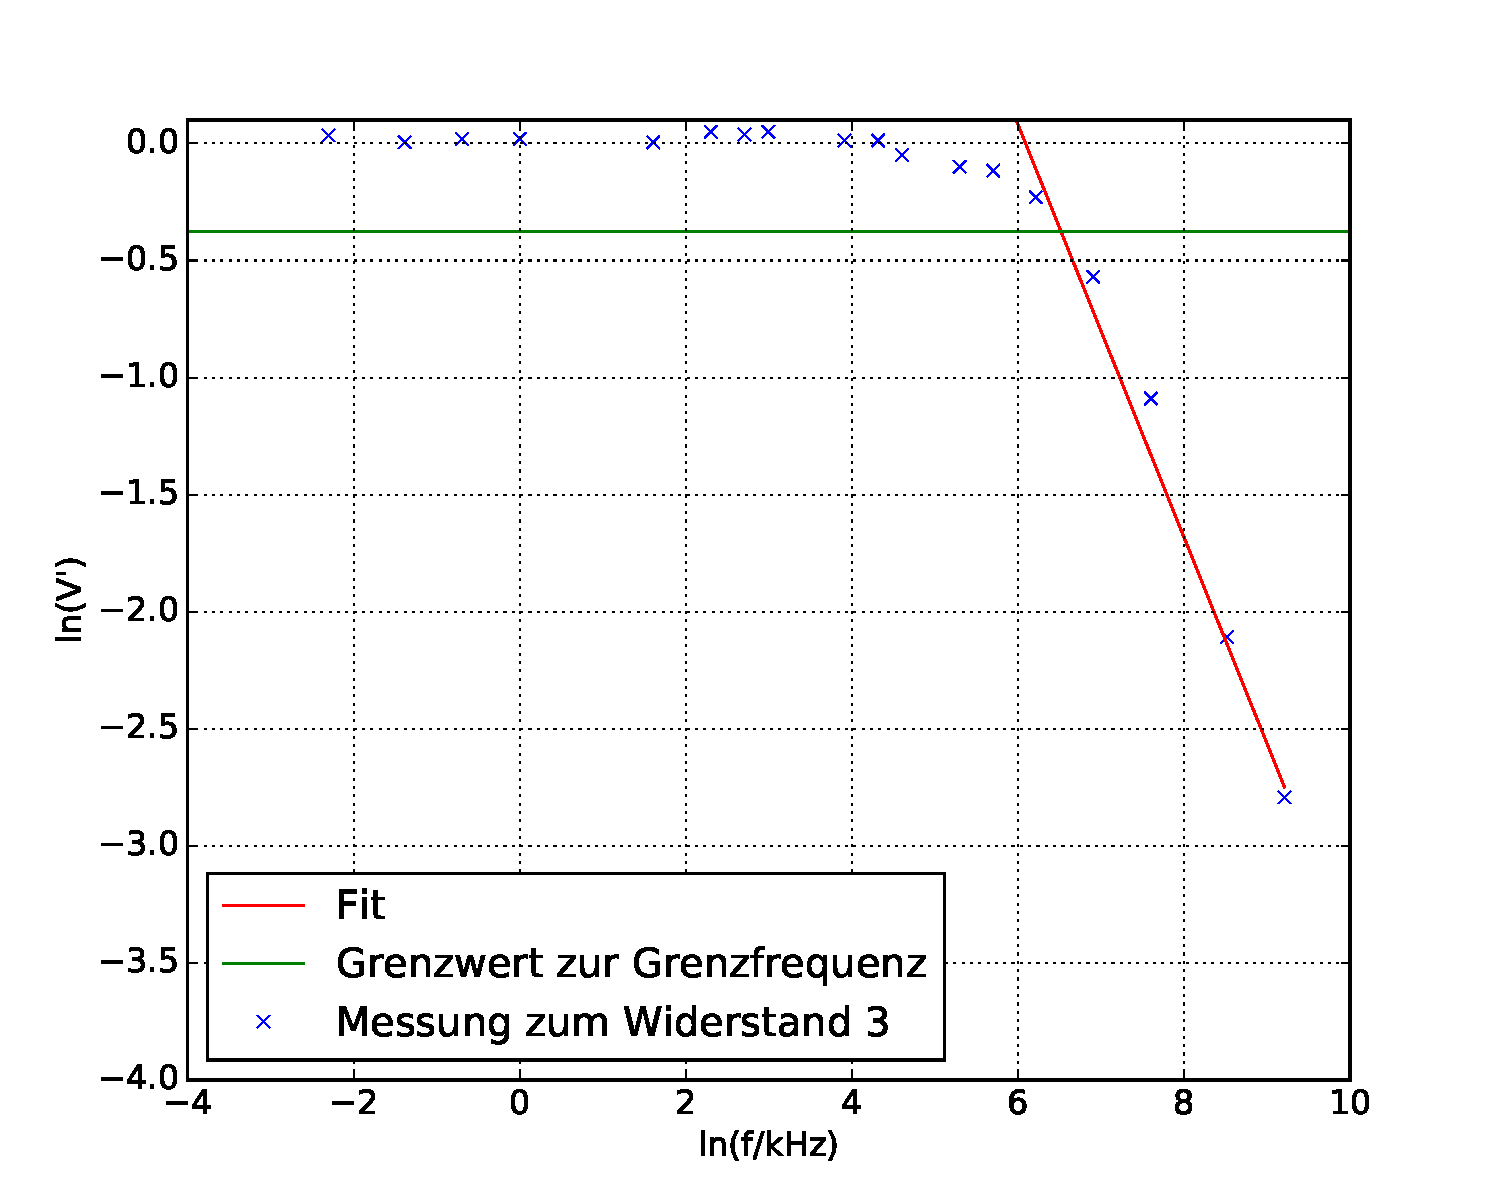
\includegraphics[width=\textwidth]{images/plot3.pdf}
	\captionof{figure}{Frequenzgang für R$_n=\SI{570}{\ohm}$}
\end{minipage}
\begin{minipage}[t]{0.5\textwidth}
	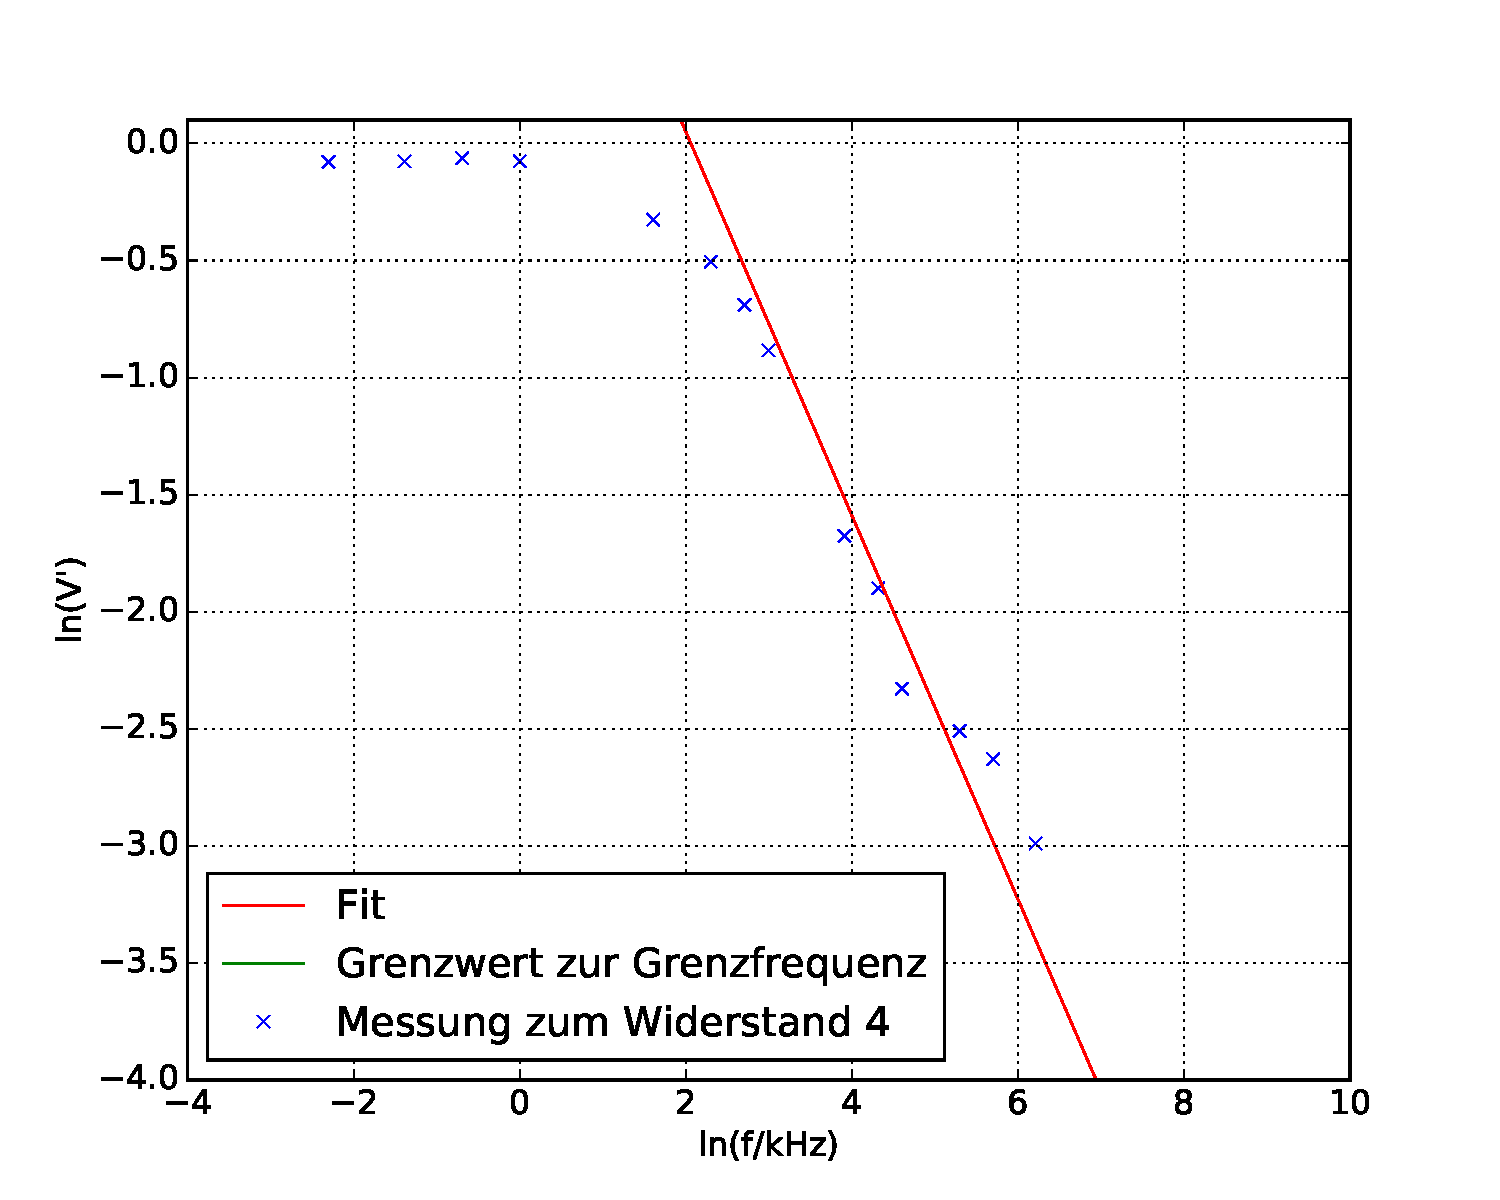
\includegraphics[width=\textwidth]{images/plot4.pdf}
	\captionof{figure}{Frequenzgang für R$_n=\SI{100}{\kilo\ohm}$}
	\label{fig:freq4}
\end{minipage} \\
\\
In Tabelle \ref{tab:frequenzgang} sind die Grenzfrequenz, die Verstärkung in Theorie und Experiment, die Leerlaufverstärkung, die Steigung m und das Verstärkungs-Bandbreite-Produkt für die einzelnen verwendeten Widerstände dargestellt. \\
\begin{table}[H]
		\captionof{table}{Experimentell bestimmte Kenndaten}
		\label{tab:frequenzgang}
		\hskip-1.50cm\begin{tabular}{r r r r r}
			\toprule
				Kenngröße & $R_n=\SI{1}{\kilo\ohm}$ & $R_n=\SI{100}{\ohm}$ &  $R_n=\SI{570}{\ohm}$ & $R_n=\SI{100}{\kilo\ohm}$ \\
			\midrule
				Grenzfrequenz f [kHz] & $450 \pm 350$ & $1000 \pm 500$ & $700 \pm 500$ & $14 \pm 11$ \\
				$V'_{ideal}$ & $1.0$ & $0.1$ & $0.57$ & $100$ \\
				$V'_{exp}$ & $0.980 \pm 0.007$ & $0.970 \pm 0.012$ & $0.970 \pm 0.012$ & $0.884 \pm 0.006$ \\
				$V'_{Leerlauf}$ & $48.25 \pm 17.04$ & $-0.111 \pm 0.000$ & $-1.38 \pm 0.02$ & $0.892 \pm 0.006$ \\
				Steigung m & $-0.860 \pm 0.070$ & $-0.897 \pm 0.046$ & $-0.882 \pm 0.070$ & $-0.819 \pm 0.098$\\
				Verstärkung-Bandbreite-Produkt [kHz] & $441.58 \pm 347.37$ & $955.89 \pm 525.67$ & $658.61 \pm 529.53$ & $12.33 \pm 9.51$ \\
			\bottomrule
		\end{tabular}
\end{table}
Die Abnahme des Ausgangsamplitude ist damit zu erklären, dass der gekoppelte Verstärker, wie in Abbildung \ref{fig:tiefpass} dargestellt, die Funktion eines Tiefpasses hat.
\begin{center}
	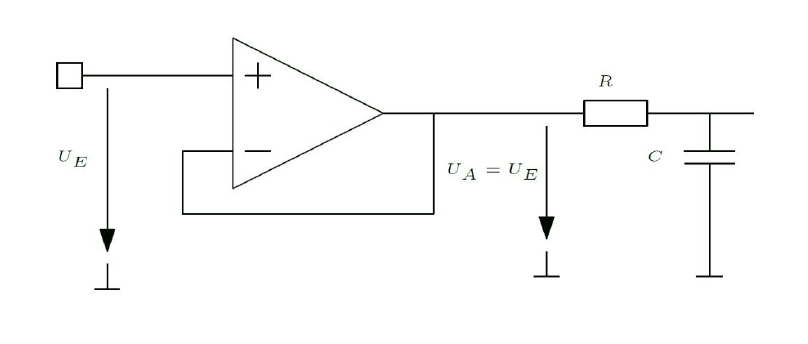
\includegraphics[width=10cm]{images/tiefpass.png}
	\captionof{figure}{Ersatzschaltbild des Tiefpasses}
	\label{fig:tiefpass}
\end{center}

\subsection{Der Umkehrintegrator}

\begin{center}
	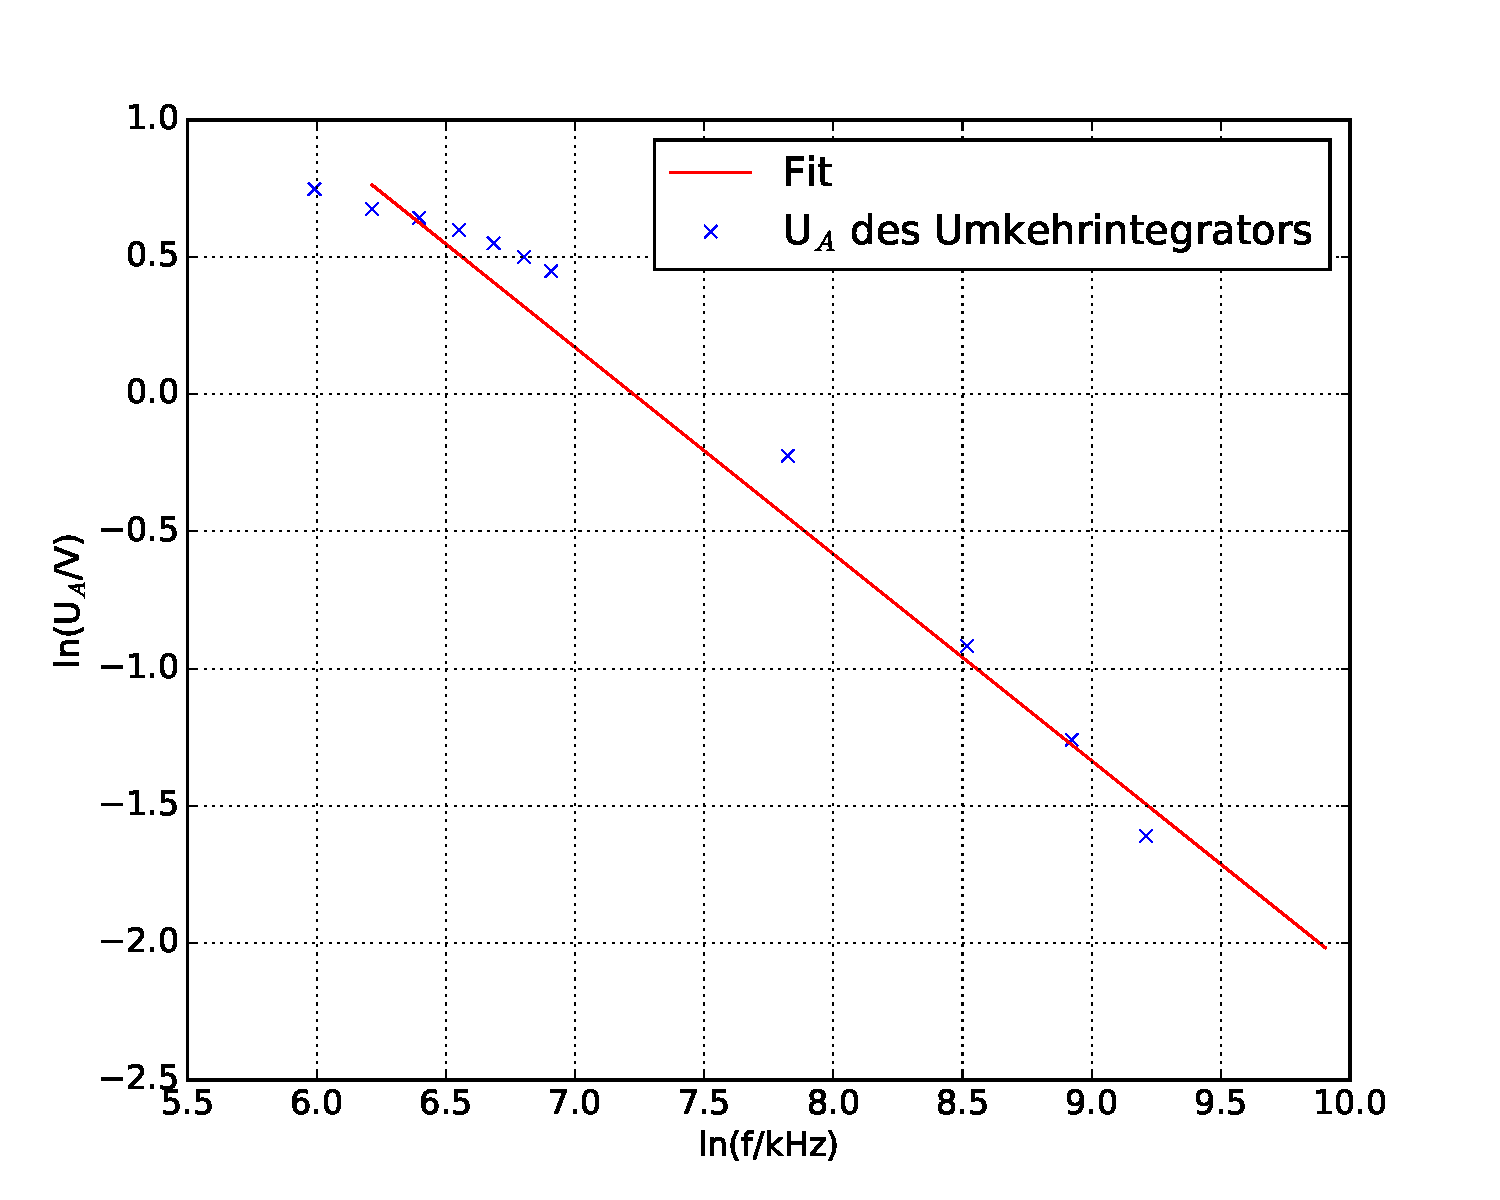
\includegraphics[width=12cm]{images/integrator.pdf}
	\captionof{figure}{Ausgangsspannung $U_A$ des Umkehrintegrators bei variierter Frequenz}
	\label{integrator}
\end{center}
\begin{minipage}[t]{0.5\textwidth}
	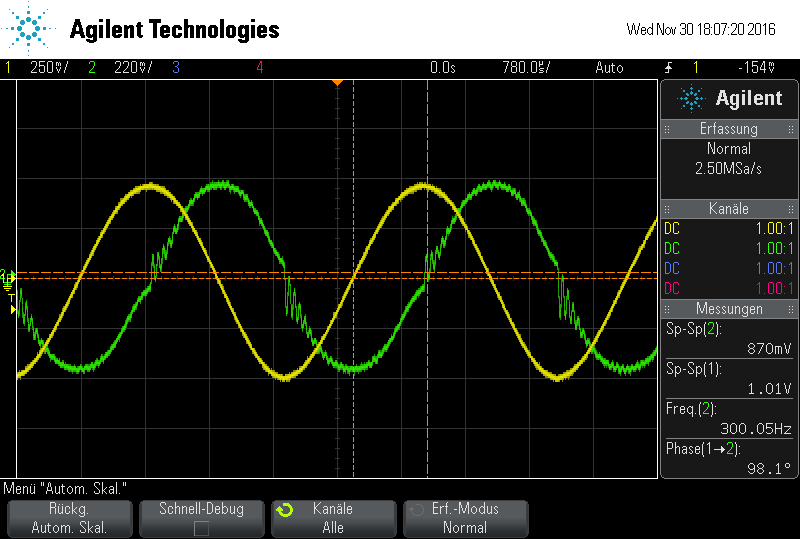
\includegraphics[width=\textwidth]{images/sinus_int}
	\captionof{figure}{Thermodruck des Signalverlaufes bei einer Sinus-Spannung}
	\label{fig:sinusint}
\end{minipage}
\hspace{0.1\textwidth}
\begin{minipage}[t]{0.5\textwidth}
	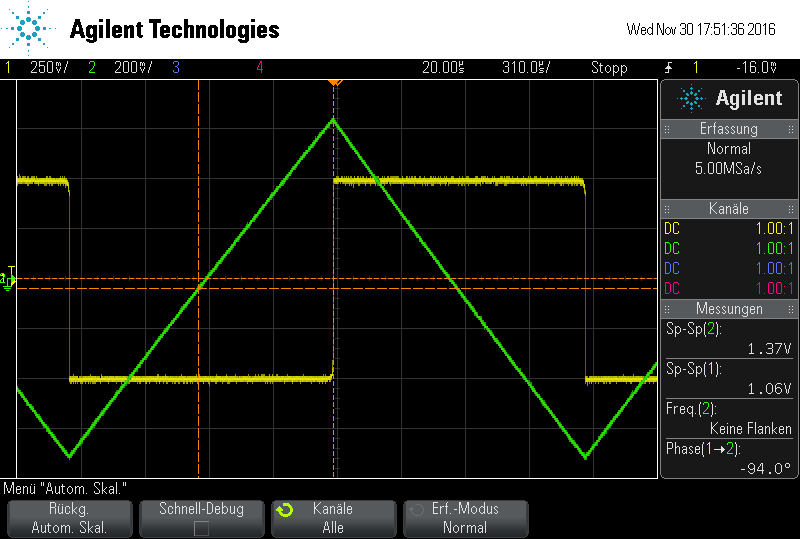
\includegraphics[width=\textwidth]{images/rechteck_int}
	\captionof{figure}{Thermodruck des Signalverlaufes bei einer Rechteck-Spannung}
	\label{fig:rechteckint}
\end{minipage} \\
\begin{minipage}[t]{0.5\textwidth}
	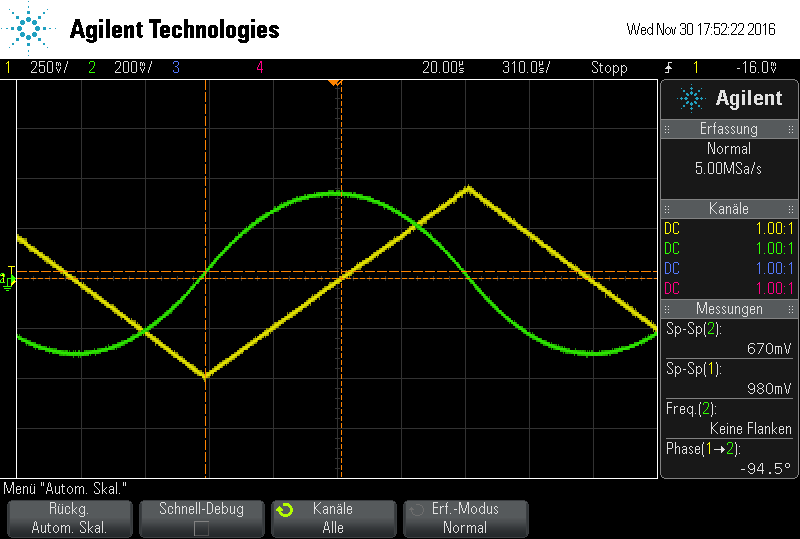
\includegraphics[width=\textwidth]{images/dreieck_int}
	\captionof{figure}{Thermodruck des Signalverlaufes bei einer Dreieck-Spannung}
	\label{fig:dreieckint}
\end{minipage}

\subsection{Der Umkehrdifferentiator}

\begin{center}
	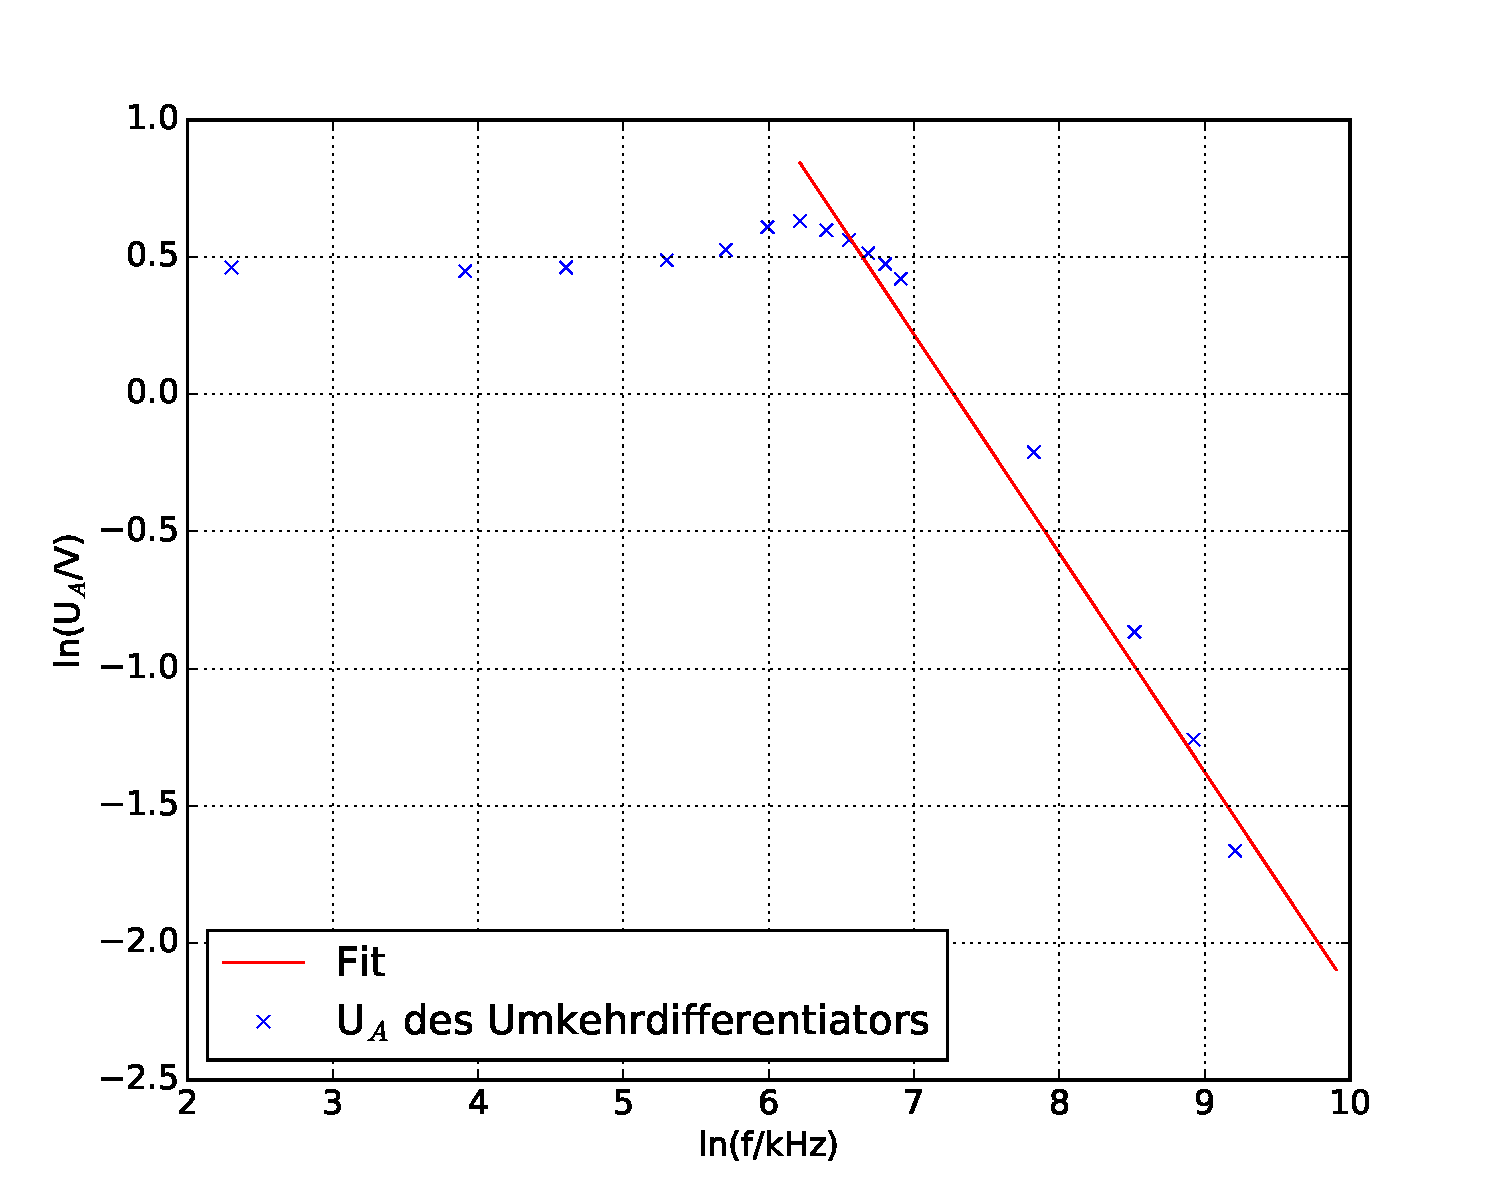
\includegraphics[width=12cm]{images/differentiator.pdf}
	\captionof{figure}{Ausgangsspannung $U_A$ des Umkehrdifferentiators bei variierter Frequenz}
	\label{differentiator}
\end{center}
\begin{minipage}[t]{0.5\textwidth}
	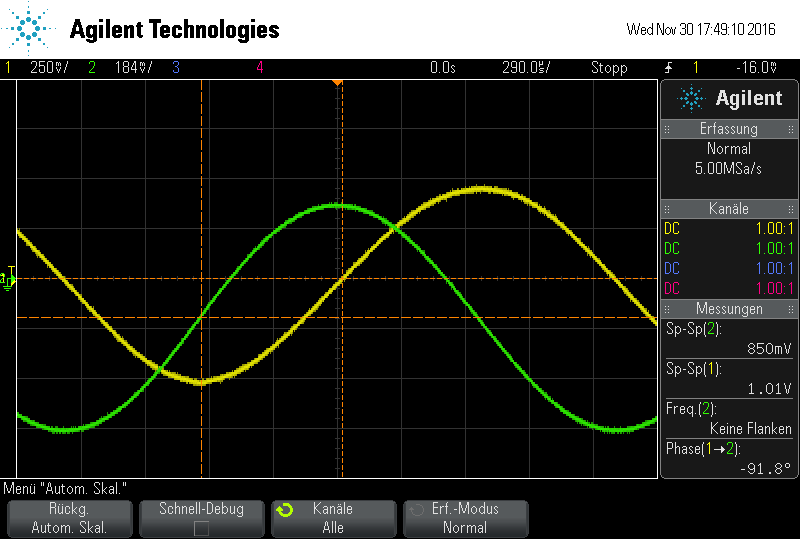
\includegraphics[width=\textwidth]{images/sinus_diff}
	\captionof{figure}{Thermodruck des Signalverlaufes bei einer Sinus-Spannung}
	\label{fig:sinusdiff}
\end{minipage}
\hspace{0.1\textwidth}
\begin{minipage}[t]{0.5\textwidth}
	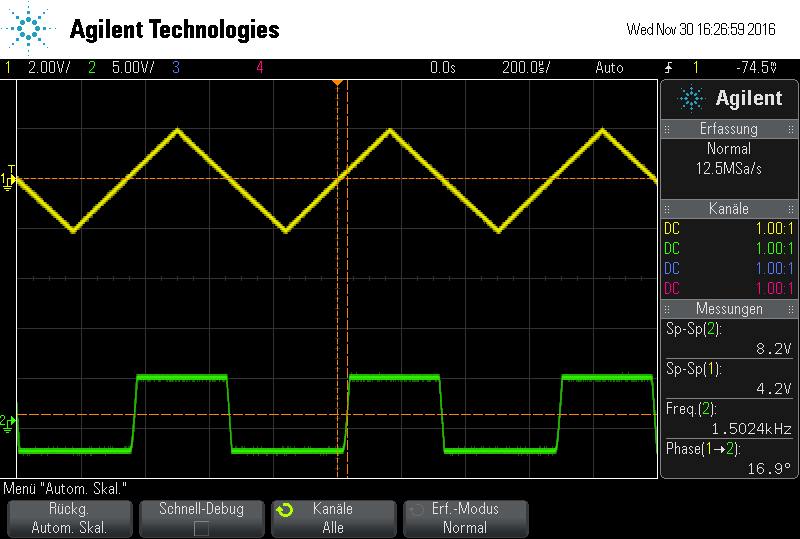
\includegraphics[width=\textwidth]{images/rechteck_diff}
	\captionof{figure}{Thermodruck des Signalverlaufes bei einer Rechteck-Spannung}
	\label{fig:rechteckdiff}
\end{minipage} \\
\begin{minipage}[t]{0.5\textwidth}
	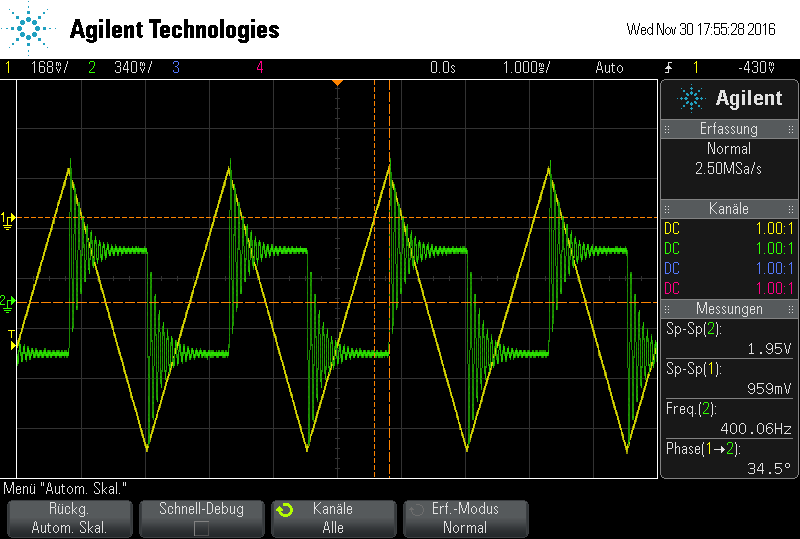
\includegraphics[width=\textwidth]{images/dreieck_diff}
	\captionof{figure}{Thermodruck des Signalverlaufes bei einer Dreieck-Spannung}
	\label{fig:dreieckdiff}
\end{minipage} 

\subsection{Der Schmitt-Trigger}

\subsection{Der Dreiecksgenerator}

\subsection{Die Schwingungsdifferentialschaltung}

\subsection{Phasenbeziehung des gegengekoppelten Verstärkers}

\section{Diskussion}

\subsection{Frequenzgang des gegengekoppelten Verstärkers}

\subsection{Der Umkehrintegrator}

\subsection{Der Umkehrdifferentiator}

\subsection{Der Schmitt-Trigger}

\subsection{Der Dreiecksgenerator}

\subsection{Die Schwingungsdifferentialschaltung}

\subsection{Phasenbeziehung des gegengekoppelten Verstärkers}

\section{Quellen}
{[1]} Versuchsanleitung zu Versuch 59: \\
http://129.217.
224.2/HOMEPAGE/PHYSIKER/MASTER/SKRIPT/V59.pdf (letzte Version vom 30.05.2016, 10:50)\\
\end{document}